\begin{figure}[H]
  \begin{center}
    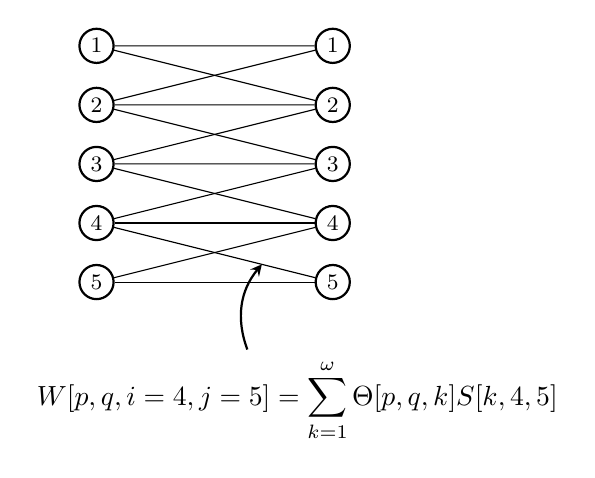
\begin{tikzpicture}[scale=1.5]
      \tikzstyle{every node} = [draw, circle, thick, inner sep = 2pt]
      
        \foreach \y in {0,...,4}{
          \pgfmathtruncatemacro{\yplusone}{5 - \y}

          \node(a\y) at (0,.5*\y) {\footnotesize\yplusone};
      }
        \foreach \y in {0,...,4}{
          \pgfmathtruncatemacro{\yplusone}{5 - \y}
                  
          \node(\y) at (2,.5*\y) {\footnotesize\yplusone};
      }
      \path
      (a0) edge (0)
      (a0) edge (1);
      \path
      (a1) edge (0)
      (a1) edge (1)
      (a1) edge (2);
      \path
      (a2) edge (1)
      (a2) edge (2)
      (a2) edge (3);
      \path
      (a3) edge (2)
      (a3) edge (3)
      (a3) edge (4);
      \path
      (a4) edge (3)
      (a4) edge (4);

      \tikzstyle{every node} = []
      \node(label) at (1.7,-1) {$W[p,q,i=4,j=5] = \displaystyle{\sum_{k=1}^{\omega}{\Theta[p,q,k] S[k,4,5]}}$};
      \path[>=stealth, ->, thick]
      (label) edge[bend left] (1.4,0.15);
    \end{tikzpicture}
  \end{center}
  \caption{Example of a propagation graph $P$ for a given input channel $p$ and feature map $q$. The edge $4 \sim 5$ is labelled with a linear combination of kernel weights from $\Theta[p,q,:]$. In the usual case, $S[k,4,5]$ is a one-hot vector that selects a single kernel weight: $\exists h, W[p,q,4,5] = \Theta[p,q,h]$.}
  \label{fig:ternary}
\end{figure}